\documentclass[]{article}
\usepackage{lmodern}
\usepackage{amssymb,amsmath}
\usepackage{ifxetex,ifluatex}
\usepackage{fixltx2e} % provides \textsubscript
\ifnum 0\ifxetex 1\fi\ifluatex 1\fi=0 % if pdftex
  \usepackage[T1]{fontenc}
  \usepackage[utf8]{inputenc}
\else % if luatex or xelatex
  \ifxetex
    \usepackage{mathspec}
  \else
    \usepackage{fontspec}
  \fi
  \defaultfontfeatures{Ligatures=TeX,Scale=MatchLowercase}
\fi
% use upquote if available, for straight quotes in verbatim environments
\IfFileExists{upquote.sty}{\usepackage{upquote}}{}
% use microtype if available
\IfFileExists{microtype.sty}{%
\usepackage{microtype}
\UseMicrotypeSet[protrusion]{basicmath} % disable protrusion for tt fonts
}{}
\usepackage[margin=1in]{geometry}
\usepackage{hyperref}
\hypersetup{unicode=true,
            pdftitle={Análise Discriminante Múltipla},
            pdfauthor={Felipe N. S. Bezerra},
            pdfborder={0 0 0},
            breaklinks=true}
\urlstyle{same}  % don't use monospace font for urls
\usepackage{color}
\usepackage{fancyvrb}
\newcommand{\VerbBar}{|}
\newcommand{\VERB}{\Verb[commandchars=\\\{\}]}
\DefineVerbatimEnvironment{Highlighting}{Verbatim}{commandchars=\\\{\}}
% Add ',fontsize=\small' for more characters per line
\usepackage{framed}
\definecolor{shadecolor}{RGB}{248,248,248}
\newenvironment{Shaded}{\begin{snugshade}}{\end{snugshade}}
\newcommand{\KeywordTok}[1]{\textcolor[rgb]{0.13,0.29,0.53}{\textbf{#1}}}
\newcommand{\DataTypeTok}[1]{\textcolor[rgb]{0.13,0.29,0.53}{#1}}
\newcommand{\DecValTok}[1]{\textcolor[rgb]{0.00,0.00,0.81}{#1}}
\newcommand{\BaseNTok}[1]{\textcolor[rgb]{0.00,0.00,0.81}{#1}}
\newcommand{\FloatTok}[1]{\textcolor[rgb]{0.00,0.00,0.81}{#1}}
\newcommand{\ConstantTok}[1]{\textcolor[rgb]{0.00,0.00,0.00}{#1}}
\newcommand{\CharTok}[1]{\textcolor[rgb]{0.31,0.60,0.02}{#1}}
\newcommand{\SpecialCharTok}[1]{\textcolor[rgb]{0.00,0.00,0.00}{#1}}
\newcommand{\StringTok}[1]{\textcolor[rgb]{0.31,0.60,0.02}{#1}}
\newcommand{\VerbatimStringTok}[1]{\textcolor[rgb]{0.31,0.60,0.02}{#1}}
\newcommand{\SpecialStringTok}[1]{\textcolor[rgb]{0.31,0.60,0.02}{#1}}
\newcommand{\ImportTok}[1]{#1}
\newcommand{\CommentTok}[1]{\textcolor[rgb]{0.56,0.35,0.01}{\textit{#1}}}
\newcommand{\DocumentationTok}[1]{\textcolor[rgb]{0.56,0.35,0.01}{\textbf{\textit{#1}}}}
\newcommand{\AnnotationTok}[1]{\textcolor[rgb]{0.56,0.35,0.01}{\textbf{\textit{#1}}}}
\newcommand{\CommentVarTok}[1]{\textcolor[rgb]{0.56,0.35,0.01}{\textbf{\textit{#1}}}}
\newcommand{\OtherTok}[1]{\textcolor[rgb]{0.56,0.35,0.01}{#1}}
\newcommand{\FunctionTok}[1]{\textcolor[rgb]{0.00,0.00,0.00}{#1}}
\newcommand{\VariableTok}[1]{\textcolor[rgb]{0.00,0.00,0.00}{#1}}
\newcommand{\ControlFlowTok}[1]{\textcolor[rgb]{0.13,0.29,0.53}{\textbf{#1}}}
\newcommand{\OperatorTok}[1]{\textcolor[rgb]{0.81,0.36,0.00}{\textbf{#1}}}
\newcommand{\BuiltInTok}[1]{#1}
\newcommand{\ExtensionTok}[1]{#1}
\newcommand{\PreprocessorTok}[1]{\textcolor[rgb]{0.56,0.35,0.01}{\textit{#1}}}
\newcommand{\AttributeTok}[1]{\textcolor[rgb]{0.77,0.63,0.00}{#1}}
\newcommand{\RegionMarkerTok}[1]{#1}
\newcommand{\InformationTok}[1]{\textcolor[rgb]{0.56,0.35,0.01}{\textbf{\textit{#1}}}}
\newcommand{\WarningTok}[1]{\textcolor[rgb]{0.56,0.35,0.01}{\textbf{\textit{#1}}}}
\newcommand{\AlertTok}[1]{\textcolor[rgb]{0.94,0.16,0.16}{#1}}
\newcommand{\ErrorTok}[1]{\textcolor[rgb]{0.64,0.00,0.00}{\textbf{#1}}}
\newcommand{\NormalTok}[1]{#1}
\usepackage{graphicx,grffile}
\makeatletter
\def\maxwidth{\ifdim\Gin@nat@width>\linewidth\linewidth\else\Gin@nat@width\fi}
\def\maxheight{\ifdim\Gin@nat@height>\textheight\textheight\else\Gin@nat@height\fi}
\makeatother
% Scale images if necessary, so that they will not overflow the page
% margins by default, and it is still possible to overwrite the defaults
% using explicit options in \includegraphics[width, height, ...]{}
\setkeys{Gin}{width=\maxwidth,height=\maxheight,keepaspectratio}
\IfFileExists{parskip.sty}{%
\usepackage{parskip}
}{% else
\setlength{\parindent}{0pt}
\setlength{\parskip}{6pt plus 2pt minus 1pt}
}
\setlength{\emergencystretch}{3em}  % prevent overfull lines
\providecommand{\tightlist}{%
  \setlength{\itemsep}{0pt}\setlength{\parskip}{0pt}}
\setcounter{secnumdepth}{0}
% Redefines (sub)paragraphs to behave more like sections
\ifx\paragraph\undefined\else
\let\oldparagraph\paragraph
\renewcommand{\paragraph}[1]{\oldparagraph{#1}\mbox{}}
\fi
\ifx\subparagraph\undefined\else
\let\oldsubparagraph\subparagraph
\renewcommand{\subparagraph}[1]{\oldsubparagraph{#1}\mbox{}}
\fi

%%% Use protect on footnotes to avoid problems with footnotes in titles
\let\rmarkdownfootnote\footnote%
\def\footnote{\protect\rmarkdownfootnote}

%%% Change title format to be more compact
\usepackage{titling}

% Create subtitle command for use in maketitle
\newcommand{\subtitle}[1]{
  \posttitle{
    \begin{center}\large#1\end{center}
    }
}

\setlength{\droptitle}{-2em}

  \title{Análise Discriminante Múltipla}
    \pretitle{\vspace{\droptitle}\centering\huge}
  \posttitle{\par}
    \author{Felipe N. S. Bezerra}
    \preauthor{\centering\large\emph}
  \postauthor{\par}
      \predate{\centering\large\emph}
  \postdate{\par}
    \date{10 de dezembro de 2018}


\begin{document}
\maketitle

Avaliação - Estatística Multivariada IV Análise Discriminante Múltipla

Considere o conjunto Auto data do pacote ISLR do software R para
desenvolver um modelo de predição para prever se um carro tem alta ou
baixa quilometragem.

\begin{Shaded}
\begin{Highlighting}[]
\KeywordTok{library}\NormalTok{(ISLR)}
\KeywordTok{library}\NormalTok{(foreign)}
\KeywordTok{library}\NormalTok{(MASS)}
\KeywordTok{library}\NormalTok{(dplyr)}
\end{Highlighting}
\end{Shaded}

\begin{verbatim}
## 
## Attaching package: 'dplyr'
\end{verbatim}

\begin{verbatim}
## The following object is masked from 'package:MASS':
## 
##     select
\end{verbatim}

\begin{verbatim}
## The following objects are masked from 'package:stats':
## 
##     filter, lag
\end{verbatim}

\begin{verbatim}
## The following objects are masked from 'package:base':
## 
##     intersect, setdiff, setequal, union
\end{verbatim}

\begin{Shaded}
\begin{Highlighting}[]
\KeywordTok{library}\NormalTok{(biotools)}
\end{Highlighting}
\end{Shaded}

\begin{verbatim}
## Loading required package: rpanel
\end{verbatim}

\begin{verbatim}
## Loading required package: tcltk
\end{verbatim}

\begin{verbatim}
## Package `rpanel', version 1.1-4: type help(rpanel) for summary information
\end{verbatim}

\begin{verbatim}
## Loading required package: tkrplot
\end{verbatim}

\begin{verbatim}
## Loading required package: lattice
\end{verbatim}

\begin{verbatim}
## Loading required package: SpatialEpi
\end{verbatim}

\begin{verbatim}
## Loading required package: sp
\end{verbatim}

\begin{verbatim}
## ---
## biotools version 3.1
\end{verbatim}

\begin{verbatim}
## 
\end{verbatim}

\begin{Shaded}
\begin{Highlighting}[]
\KeywordTok{library}\NormalTok{(DiscriMiner)}
\KeywordTok{library}\NormalTok{(ggplot2)}
\KeywordTok{library}\NormalTok{(mvnormtest)}
\end{Highlighting}
\end{Shaded}

\begin{Shaded}
\begin{Highlighting}[]
\KeywordTok{summary}\NormalTok{(Auto)}
\end{Highlighting}
\end{Shaded}

\begin{verbatim}
##       mpg          cylinders      displacement     horsepower   
##  Min.   : 9.00   Min.   :3.000   Min.   : 68.0   Min.   : 46.0  
##  1st Qu.:17.00   1st Qu.:4.000   1st Qu.:105.0   1st Qu.: 75.0  
##  Median :22.75   Median :4.000   Median :151.0   Median : 93.5  
##  Mean   :23.45   Mean   :5.472   Mean   :194.4   Mean   :104.5  
##  3rd Qu.:29.00   3rd Qu.:8.000   3rd Qu.:275.8   3rd Qu.:126.0  
##  Max.   :46.60   Max.   :8.000   Max.   :455.0   Max.   :230.0  
##                                                                 
##      weight      acceleration        year           origin     
##  Min.   :1613   Min.   : 8.00   Min.   :70.00   Min.   :1.000  
##  1st Qu.:2225   1st Qu.:13.78   1st Qu.:73.00   1st Qu.:1.000  
##  Median :2804   Median :15.50   Median :76.00   Median :1.000  
##  Mean   :2978   Mean   :15.54   Mean   :75.98   Mean   :1.577  
##  3rd Qu.:3615   3rd Qu.:17.02   3rd Qu.:79.00   3rd Qu.:2.000  
##  Max.   :5140   Max.   :24.80   Max.   :82.00   Max.   :3.000  
##                                                                
##                  name    
##  amc matador       :  5  
##  ford pinto        :  5  
##  toyota corolla    :  5  
##  amc gremlin       :  4  
##  amc hornet        :  4  
##  chevrolet chevette:  4  
##  (Other)           :365
\end{verbatim}

\begin{verbatim}
(a) Crie uma variável binária, classmpg, que seja igual a 1 se o mpg for maior do que a mediana e 0, caso contrário. Você pode calcular a mediana de mpg no R usando a função median(). Note que talvez seja mais fácil usar o comando data.frame() para criar um conjunto de dados que contenha o classmpg e as demais variáveis do Auto data.
\end{verbatim}

\begin{Shaded}
\begin{Highlighting}[]
\NormalTok{avaldata <-}\StringTok{ }\NormalTok{Auto[,}\OperatorTok{-}\DecValTok{1}\NormalTok{]}
\NormalTok{avaldata <-}\StringTok{ }\NormalTok{avaldata[,}\OperatorTok{-}\DecValTok{8}\NormalTok{]}
\NormalTok{avaldata}\OperatorTok{$}\NormalTok{origin <-}\StringTok{ }\KeywordTok{as.factor}\NormalTok{(avaldata}\OperatorTok{$}\NormalTok{origin)}

\NormalTok{scaleavaldata <-}\StringTok{ }\NormalTok{avaldata[,}\OperatorTok{-}\DecValTok{7}\NormalTok{]}
\NormalTok{scaleavaldata <-}\StringTok{ }\KeywordTok{as.data.frame}\NormalTok{(}\KeywordTok{scale}\NormalTok{(scaleavaldata))}

\NormalTok{classmpg <-}\StringTok{ }\KeywordTok{as.numeric}\NormalTok{(Auto}\OperatorTok{$}\NormalTok{mpg}\OperatorTok{>}\KeywordTok{median}\NormalTok{(Auto}\OperatorTok{$}\NormalTok{mpg))}
\NormalTok{avaldata}\OperatorTok{$}\NormalTok{classmpg <-}\StringTok{ }\KeywordTok{as.factor}\NormalTok{(classmpg)}
\NormalTok{scaleavaldata}\OperatorTok{$}\NormalTok{origin <-}\StringTok{ }\NormalTok{avaldata}\OperatorTok{$}\NormalTok{origin}
\NormalTok{scaleavaldata}\OperatorTok{$}\NormalTok{classmpg <-}\StringTok{ }\NormalTok{avaldata}\OperatorTok{$}\NormalTok{classmpg}
\end{Highlighting}
\end{Shaded}

\begin{center}\rule{0.5\linewidth}{\linethickness}\end{center}

\begin{verbatim}
(b) Explore os dados graficamente para investigar a associação entre o classmpg e as demais variáveis. Quais variáveis parecem ser úteis para prever o classmpg? Pode usar boxplots para responder a essa questão.
\end{verbatim}

\begin{Shaded}
\begin{Highlighting}[]
\KeywordTok{boxplot}\NormalTok{(avaldata}\OperatorTok{$}\NormalTok{cylinders }\OperatorTok{~}\StringTok{ }\NormalTok{avaldata}\OperatorTok{$}\NormalTok{classmpg, }\DataTypeTok{main=}\StringTok{'Cilindros'}\NormalTok{)}
\end{Highlighting}
\end{Shaded}

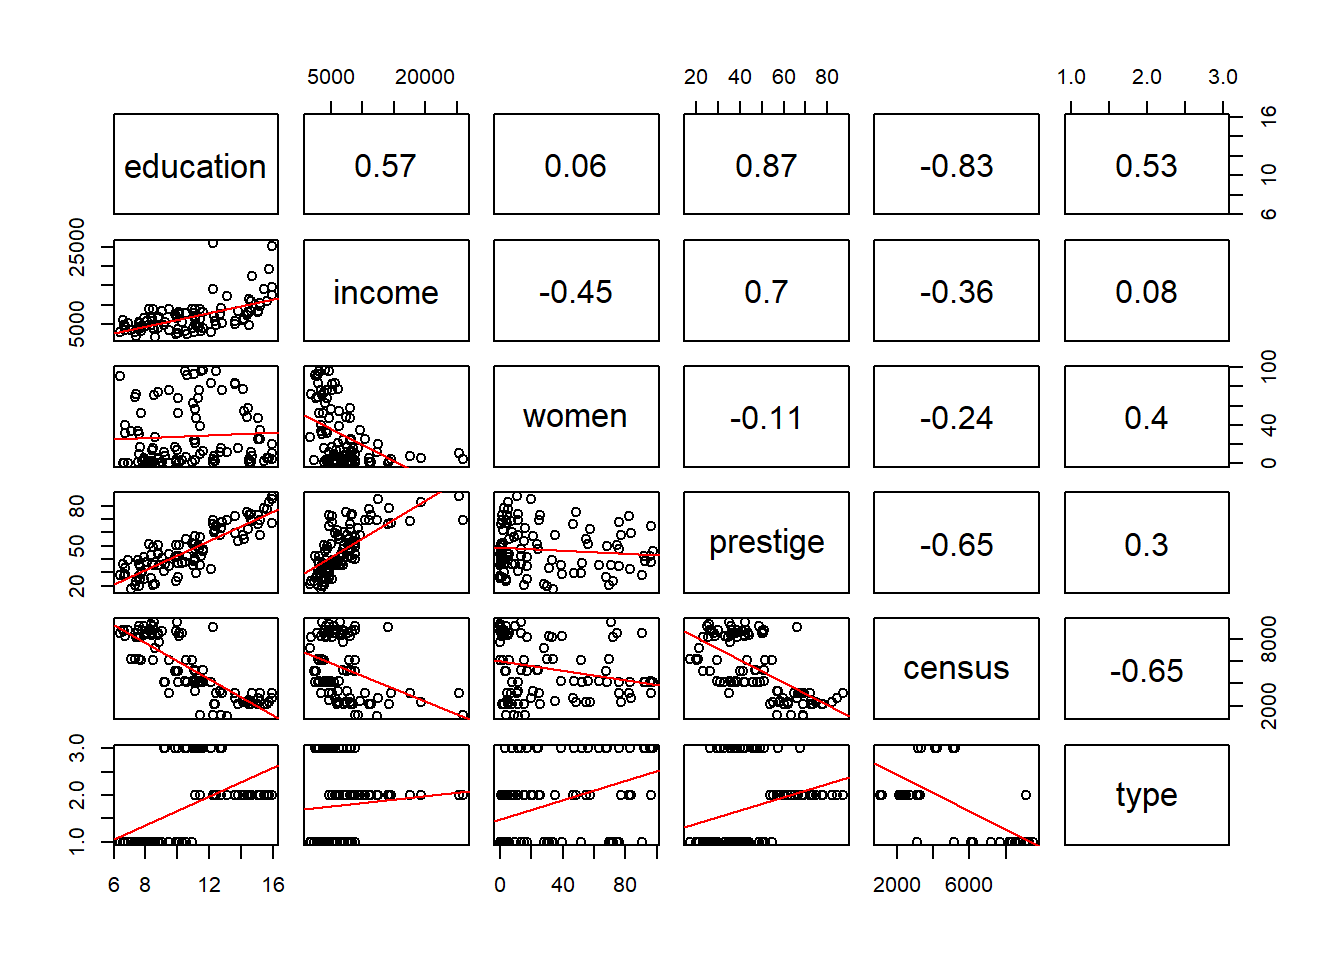
\includegraphics{Avaliação_-_Felipe_Neres_files/figure-latex/unnamed-chunk-4-1.pdf}

\begin{Shaded}
\begin{Highlighting}[]
\KeywordTok{boxplot}\NormalTok{(avaldata}\OperatorTok{$}\NormalTok{displacement }\OperatorTok{~}\StringTok{ }\NormalTok{avaldata}\OperatorTok{$}\NormalTok{classmpg, }\DataTypeTok{main=}\StringTok{'Deslocamento do Motor'}\NormalTok{)}
\end{Highlighting}
\end{Shaded}

\includegraphics{Avaliação_-_Felipe_Neres_files/figure-latex/unnamed-chunk-4-2.pdf}

\begin{Shaded}
\begin{Highlighting}[]
\KeywordTok{boxplot}\NormalTok{(avaldata}\OperatorTok{$}\NormalTok{horsepower }\OperatorTok{~}\StringTok{ }\NormalTok{avaldata}\OperatorTok{$}\NormalTok{classmpg, }\DataTypeTok{main=}\StringTok{'Potência')}
\end{Highlighting}
\end{Shaded}

\includegraphics{Avaliação_-_Felipe_Neres_files/figure-latex/unnamed-chunk-4-3.pdf}

\begin{Shaded}
\begin{Highlighting}[]
\KeywordTok{boxplot}\NormalTok{(avaldata}\OperatorTok{$}\NormalTok{weight }\OperatorTok{~}\StringTok{ }\NormalTok{avaldata}\OperatorTok{$}\NormalTok{classmpg, }\DataTypeTok{main=}\StringTok{'Peso'}\NormalTok{)}
\end{Highlighting}
\end{Shaded}

\includegraphics{Avaliação_-_Felipe_Neres_files/figure-latex/unnamed-chunk-4-4.pdf}

\begin{Shaded}
\begin{Highlighting}[]
\KeywordTok{boxplot}\NormalTok{(avaldata}\OperatorTok{$}\NormalTok{acceleration }\OperatorTok{~}\StringTok{ }\NormalTok{avaldata}\OperatorTok{$}\NormalTok{classmpg, }\DataTypeTok{main=}\StringTok{'Aceleração'}\NormalTok{)}
\end{Highlighting}
\end{Shaded}

\includegraphics{Avaliação_-_Felipe_Neres_files/figure-latex/unnamed-chunk-4-5.pdf}

\begin{Shaded}
\begin{Highlighting}[]
\KeywordTok{boxplot}\NormalTok{(avaldata}\OperatorTok{$}\NormalTok{year }\OperatorTok{~}\StringTok{ }\NormalTok{avaldata}\OperatorTok{$}\NormalTok{classmpg, }\DataTypeTok{main=}\StringTok{'Ano'}\NormalTok{)}
\end{Highlighting}
\end{Shaded}

\includegraphics{Avaliação_-_Felipe_Neres_files/figure-latex/unnamed-chunk-4-6.pdf}

\begin{Shaded}
\begin{Highlighting}[]
\KeywordTok{aggregate}\NormalTok{(avaldata[,}\DecValTok{1}\OperatorTok{:}\DecValTok{6}\NormalTok{], }\KeywordTok{list}\NormalTok{(avaldata}\OperatorTok{$}\NormalTok{classmpg), quantile)}
\end{Highlighting}
\end{Shaded}

\begin{verbatim}
##   Group.1 cylinders.0% cylinders.25% cylinders.50% cylinders.75%
## 1       0            3             6             8             8
## 2       1            3             4             4             4
##   cylinders.100% displacement.0% displacement.25% displacement.50%
## 1              8              70              225              261
## 2              8              68               91              105
##   displacement.75% displacement.100% horsepower.0% horsepower.25%
## 1              350               455          72.0          100.0
## 2              134               350          46.0           67.0
##   horsepower.50% horsepower.75% horsepower.100% weight.0% weight.25%
## 1          125.0          150.0           230.0   2124.00    3139.75
## 2           76.5           90.0           132.0   1613.00    2045.00
##   weight.50% weight.75% weight.100% acceleration.0% acceleration.25%
## 1    3607.00    4156.75     5140.00           8.000           12.950
## 2    2229.00    2607.50     3900.00          11.300           14.700
##   acceleration.50% acceleration.75% acceleration.100% year.0% year.25%
## 1           14.500           16.250            21.900      70       72
## 2           16.200           17.925            24.800      70       75
##   year.50% year.75% year.100%
## 1       74       77        82
## 2       78       81        82
\end{verbatim}

As variáveis ``Cilindros'' e ``Deslocamento do Motor'' parecem possuir
maior acertividade em definir os veículos com maior consumo de
combustível (classmpg = 0). Veículos com um número de cilindros
diferente de 4 e Deslocamento do Motor com mais de 200 in percorrem
menos milhas por galão; as demais faixas destas variáveis apresentam
consumo de combustível variado. Veículos com maior potência, menor
aceleração, mais pesados e mais antigos aparentam consumir mais
combustível, mas tendência não se mostra tão definida quanto as duas
variáveis citadas anteriormente.

\begin{center}\rule{0.5\linewidth}{\linethickness}\end{center}

\begin{verbatim}
(c) Divida os dados em duas amostras, uma de treino (75%) e outra de teste (25%).
\end{verbatim}

\begin{Shaded}
\begin{Highlighting}[]
\KeywordTok{set.seed}\NormalTok{(}\DecValTok{8}\NormalTok{)}
\NormalTok{treinoaval <-}\StringTok{ }\NormalTok{scaleavaldata[}\KeywordTok{sample}\NormalTok{(}\KeywordTok{nrow}\NormalTok{(scaleavaldata),  }\DataTypeTok{size =} \KeywordTok{nrow}\NormalTok{(scaleavaldata) }\OperatorTok{*}\StringTok{ }\FloatTok{0.75}\NormalTok{),]}
\NormalTok{testeaval <-}\StringTok{ }\NormalTok{scaleavaldata[}\OperatorTok{-}\KeywordTok{sample}\NormalTok{(}\KeywordTok{nrow}\NormalTok{(scaleavaldata),  }\DataTypeTok{size =} \KeywordTok{nrow}\NormalTok{(scaleavaldata) }\OperatorTok{*}\StringTok{ }\FloatTok{0.75}\NormalTok{),]}
\end{Highlighting}
\end{Shaded}

\begin{center}\rule{0.5\linewidth}{\linethickness}\end{center}

\begin{verbatim}
(d) Obtenha e interprete as funções discriminantes para esse estudo. Verifique também as suposições da análise. Você utilizaria a análise discriminante linear ou quadrática para classificação?
\end{verbatim}

Verificação do tamanho da amostra:

\begin{Shaded}
\begin{Highlighting}[]
\KeywordTok{table}\NormalTok{(scaleavaldata}\OperatorTok{$}\NormalTok{classmpg)}
\end{Highlighting}
\end{Shaded}

\begin{verbatim}
## 
##   0   1 
## 196 196
\end{verbatim}

\begin{Shaded}
\begin{Highlighting}[]
\KeywordTok{table}\NormalTok{(treinoaval}\OperatorTok{$}\NormalTok{classmpg)}
\end{Highlighting}
\end{Shaded}

\begin{verbatim}
## 
##   0   1 
## 146 148
\end{verbatim}

\begin{Shaded}
\begin{Highlighting}[]
\KeywordTok{table}\NormalTok{(testeaval}\OperatorTok{$}\NormalTok{classmpg)}
\end{Highlighting}
\end{Shaded}

\begin{verbatim}
## 
##  0  1 
## 50 48
\end{verbatim}

Todos os grupos possuem mais de 20 observações (número aceitável para 6
variáveis independentes), inclusive nas amostras separadas para treino e
teste.

Verificação de multicolinearidade:

\begin{Shaded}
\begin{Highlighting}[]
\KeywordTok{cor}\NormalTok{(scaleavaldata[,}\DecValTok{1}\OperatorTok{:}\DecValTok{6}\NormalTok{])}
\end{Highlighting}
\end{Shaded}

\begin{verbatim}
##               cylinders displacement horsepower     weight acceleration
## cylinders     1.0000000    0.9508233  0.8429834  0.8975273   -0.5046834
## displacement  0.9508233    1.0000000  0.8972570  0.9329944   -0.5438005
## horsepower    0.8429834    0.8972570  1.0000000  0.8645377   -0.6891955
## weight        0.8975273    0.9329944  0.8645377  1.0000000   -0.4168392
## acceleration -0.5046834   -0.5438005 -0.6891955 -0.4168392    1.0000000
## year         -0.3456474   -0.3698552 -0.4163615 -0.3091199    0.2903161
##                    year
## cylinders    -0.3456474
## displacement -0.3698552
## horsepower   -0.4163615
## weight       -0.3091199
## acceleration  0.2903161
## year          1.0000000
\end{verbatim}

As variáveis ``Cilindros''e ``Deslocamento do Motor'' estão altamente
correlacionadas (correlação superior a 0,95). Utilizar ambas implica em
redundância, então apenas uma (Deslocamento do Motor) será utilizada no
ajuste do modelo.

Normalidade multivariada das variáveis independentes:

\begin{Shaded}
\begin{Highlighting}[]
\KeywordTok{mshapiro.test}\NormalTok{(}\KeywordTok{t}\NormalTok{(scaleavaldata[,}\DecValTok{1}\OperatorTok{:}\DecValTok{6}\NormalTok{]))}
\end{Highlighting}
\end{Shaded}

\begin{verbatim}
## 
##  Shapiro-Wilk normality test
## 
## data:  Z
## W = 0.86677, p-value < 2.2e-16
\end{verbatim}

\begin{Shaded}
\begin{Highlighting}[]
\KeywordTok{shapiro.test}\NormalTok{(scaleavaldata}\OperatorTok{$}\NormalTok{cylinders)}
\end{Highlighting}
\end{Shaded}

\begin{verbatim}
## 
##  Shapiro-Wilk normality test
## 
## data:  scaleavaldata$cylinders
## W = 0.75066, p-value < 2.2e-16
\end{verbatim}

\begin{Shaded}
\begin{Highlighting}[]
\KeywordTok{shapiro.test}\NormalTok{(scaleavaldata}\OperatorTok{$}\NormalTok{displacement)}
\end{Highlighting}
\end{Shaded}

\begin{verbatim}
## 
##  Shapiro-Wilk normality test
## 
## data:  scaleavaldata$displacement
## W = 0.88184, p-value < 2.2e-16
\end{verbatim}

\begin{Shaded}
\begin{Highlighting}[]
\KeywordTok{shapiro.test}\NormalTok{(scaleavaldata}\OperatorTok{$}\NormalTok{horsepower)}
\end{Highlighting}
\end{Shaded}

\begin{verbatim}
## 
##  Shapiro-Wilk normality test
## 
## data:  scaleavaldata$horsepower
## W = 0.9041, p-value = 5.022e-15
\end{verbatim}

\begin{Shaded}
\begin{Highlighting}[]
\KeywordTok{shapiro.test}\NormalTok{(scaleavaldata}\OperatorTok{$}\NormalTok{weight)}
\end{Highlighting}
\end{Shaded}

\begin{verbatim}
## 
##  Shapiro-Wilk normality test
## 
## data:  scaleavaldata$weight
## W = 0.94147, p-value = 2.602e-11
\end{verbatim}

\begin{Shaded}
\begin{Highlighting}[]
\KeywordTok{shapiro.test}\NormalTok{(scaleavaldata}\OperatorTok{$}\NormalTok{acceleration)}
\end{Highlighting}
\end{Shaded}

\begin{verbatim}
## 
##  Shapiro-Wilk normality test
## 
## data:  scaleavaldata$acceleration
## W = 0.99187, p-value = 0.03053
\end{verbatim}

\begin{Shaded}
\begin{Highlighting}[]
\KeywordTok{shapiro.test}\NormalTok{(scaleavaldata}\OperatorTok{$}\NormalTok{year)}
\end{Highlighting}
\end{Shaded}

\begin{verbatim}
## 
##  Shapiro-Wilk normality test
## 
## data:  scaleavaldata$year
## W = 0.94697, p-value = 1.223e-10
\end{verbatim}

Segundo o teste de Shapiro-Wilk, nenhuma das variáveis independentes
segue distribuição normal e, consequentemente, a amostra não obedece ao
pressuposto de normalidade multivariada, requerido para que se prossiga
com a análise discriminante.

Homogeneidade de variância/covariância:

\begin{Shaded}
\begin{Highlighting}[]
\KeywordTok{boxM}\NormalTok{(}\DataTypeTok{data =}\NormalTok{ scaleavaldata[,}\DecValTok{1}\OperatorTok{:}\DecValTok{6}\NormalTok{], }\DataTypeTok{grouping =}\NormalTok{ scaleavaldata}\OperatorTok{$}\NormalTok{classmpg)}
\end{Highlighting}
\end{Shaded}

\begin{verbatim}
## 
##  Box's M-test for Homogeneity of Covariance Matrices
## 
## data:  scaleavaldata[, 1:6]
## Chi-Sq (approx.) = 404.08, df = 21, p-value < 2.2e-16
\end{verbatim}

Não há igualdade entre as matrizes de variâncias e covariâncias da
amostra, mesmo considerando aceitável um p-valor de 0,01 (mais comum
para este teste).

Seleção de variável:

\begin{Shaded}
\begin{Highlighting}[]
\KeywordTok{discPower}\NormalTok{(}\DataTypeTok{variables =}\NormalTok{ treinoaval[,}\DecValTok{1}\OperatorTok{:}\DecValTok{6}\NormalTok{], }\DataTypeTok{group =}\NormalTok{ treinoaval}\OperatorTok{$}\NormalTok{classmpg)}
\end{Highlighting}
\end{Shaded}

\begin{verbatim}
##              correl_ratio wilks_lambda F_statistic      p_value
## cylinders       0.5610599    0.4389401   373.23890 0.000000e+00
## displacement    0.5495676    0.4504324   356.26593 0.000000e+00
## horsepower      0.4354455    0.5645545   225.22203 0.000000e+00
## weight          0.5725786    0.4274214   391.16648 0.000000e+00
## acceleration    0.1017403    0.8982597    33.07302 2.236779e-08
## year            0.1996819    0.8003181    72.85494 7.771561e-16
\end{verbatim}

\begin{verbatim}
         correl_ratio wilks_lambda F_statistic      p_value
\end{verbatim}

cylinders 0.5610599 0.4389401 373.23890 0.000000e+00 \textbf{\emph{
displacement 0.5495676 0.4504324 356.26593 0.000000e+00 }} horsepower
0.4354455 0.5645545 225.22203 0.000000e+00 \textbf{\emph{ weight
0.5725786 0.4274214 391.16648 0.000000e+00 }} acceleration 0.1017403
0.8982597 33.07302 2.236779e-08 \textbf{\emph{ year 0.1996819 0.8003181
72.85494 7.771561e-16 }}

Todas as variáveis contribuem significativamente para a discriminação
dos grupos (embora com menor relevância se tratando da ``Aceleração'' e
do ``Ano do Modelo'').

Determinação da função discriminante:

\begin{Shaded}
\begin{Highlighting}[]
\NormalTok{discrim_aval <-}\StringTok{ }\KeywordTok{desDA}\NormalTok{(}\DataTypeTok{variables =}\NormalTok{ treinoaval[, }\KeywordTok{c}\NormalTok{(}\StringTok{"displacement"}\NormalTok{, }\StringTok{"horsepower"}\NormalTok{, }\StringTok{"weight"}\NormalTok{, }\StringTok{"acceleration"}\NormalTok{, }\StringTok{"year"}\NormalTok{)], }
                   \DataTypeTok{group =}\NormalTok{ treinoaval}\OperatorTok{$}\NormalTok{classmpg)}
\end{Highlighting}
\end{Shaded}

Coeficientes das funções discriminantes:

\begin{Shaded}
\begin{Highlighting}[]
\NormalTok{discrim_aval}\OperatorTok{$}\NormalTok{discrivar}
\end{Highlighting}
\end{Shaded}

\begin{verbatim}
##                       DF1
## constant     -0.004868575
## displacement -0.606862514
## horsepower    0.467179185
## weight       -1.262871937
## acceleration  0.033320876
## year          0.477663363
\end{verbatim}

Como há apenas dois grupos, só é necessária uma função discriminante.
\(DF= -0,005 -0,607*displacement +0,467*horsepower -1,263*weight +0,033*acceleration +0,478*year\)

Autovalores das funções discriminantes e variabilidade explicada:

\begin{Shaded}
\begin{Highlighting}[]
\NormalTok{discrim_aval}\OperatorTok{$}\NormalTok{values}
\end{Highlighting}
\end{Shaded}

\begin{verbatim}
##        value proportion accumulated
## DF1 1.699744        100         100
\end{verbatim}

Como só há uma função discriminante, toda a variância do modelo é
explicada por ela.

Matriz de fatores (correlação entre as variáveis explicativas e a função
discriminante):

\begin{Shaded}
\begin{Highlighting}[]
\NormalTok{discrim_aval}\OperatorTok{$}\NormalTok{discor}
\end{Highlighting}
\end{Shaded}

\begin{verbatim}
##                     DF1
## displacement -0.9342946
## horsepower   -0.8316493
## weight       -0.9536540
## acceleration  0.4019941
## year          0.5631741
\end{verbatim}

A função discriminante obtida é mais fortemente ponderada pelo ``Peso do
Veídulo'' e pelo ``Deslocamento do motor'', e menos pela ``Aceleração''
e pelo ``Ano do Modelo''.

Significância da função discriminante

\begin{Shaded}
\begin{Highlighting}[]
\KeywordTok{summary}\NormalTok{(}\KeywordTok{aov}\NormalTok{(discrim_aval}\OperatorTok{$}\NormalTok{scores }\OperatorTok{~}\StringTok{ }\NormalTok{treinoaval}\OperatorTok{$}\NormalTok{classmpg), }\DataTypeTok{test=}\StringTok{"Wilks"}\NormalTok{)}
\end{Highlighting}
\end{Shaded}

\begin{verbatim}
##                      Df Sum Sq Mean Sq F value Pr(>F)    
## treinoaval$classmpg   1  496.3   496.3   496.3 <2e-16 ***
## Residuals           292  292.0     1.0                   
## ---
## Signif. codes:  0 '***' 0.001 '**' 0.01 '*' 0.05 '.' 0.1 ' ' 1
\end{verbatim}

Dado o baixo p-valor, a função é considerada significante.

Centróide:

\begin{Shaded}
\begin{Highlighting}[]
\NormalTok{treinoaval}\OperatorTok{$}\NormalTok{DF1 <-}\StringTok{ }\NormalTok{discrim_aval}\OperatorTok{$}\NormalTok{scores}
\NormalTok{treinoaval }\OperatorTok\StringTok{ }\KeywordTok{group_by}\NormalTok{(classmpg) }\OperatorTok\StringTok{ }\KeywordTok{summarise}\NormalTok{(}\DataTypeTok{C =} \KeywordTok{mean}\NormalTok{(DF1))}
\end{Highlighting}
\end{Shaded}

\begin{verbatim}
## # A tibble: 2 x 2
##   classmpg     C
##   <fct>    <dbl>
## 1 0        -1.31
## 2 1         1.29
\end{verbatim}

\section{A tibble: 2 x 2}\label{a-tibble-2-x-2}

classmpg C 1 0 -1.31 2 1 1.29

A função discriminante é desenvolvida de modo a tornar os valores do
grupo dos veículos com maior consumo de combustível (classmpg = 0)
negativos e do grupo dos veículos com menor consumo (classmpg = 1)
positivos; isso fica explícito pelos valores discriminantes dos
centróides de cada grupo

Scatterplot

\begin{Shaded}
\begin{Highlighting}[]
\NormalTok{treinoaval}\OperatorTok{$}\NormalTok{random <-}\StringTok{ }\KeywordTok{rnorm}\NormalTok{(}\DecValTok{294}\NormalTok{,}\DataTypeTok{mean=}\DecValTok{0}\NormalTok{,}\DataTypeTok{sd=}\DecValTok{10}\NormalTok{)}

\KeywordTok{library}\NormalTok{(ggplot2)}
\KeywordTok{ggplot}\NormalTok{(}\DataTypeTok{data =}\NormalTok{ treinoaval, }\KeywordTok{aes}\NormalTok{(}\DataTypeTok{x =}\NormalTok{ DF1, }\DataTypeTok{y =}\NormalTok{ random, }\DataTypeTok{colour =}\NormalTok{ classmpg)) }\OperatorTok{+}
\StringTok{  }\KeywordTok{geom_hline}\NormalTok{(}\DataTypeTok{yintercept =} \DecValTok{0}\NormalTok{, }\DataTypeTok{colour=}\StringTok{"gray70"}\NormalTok{) }\OperatorTok{+}
\StringTok{  }\KeywordTok{geom_vline}\NormalTok{(}\DataTypeTok{xintercept =} \DecValTok{0}\NormalTok{, }\DataTypeTok{colour=}\StringTok{"gray70"}\NormalTok{) }\OperatorTok{+}
\StringTok{  }\KeywordTok{geom_point}\NormalTok{()}
\end{Highlighting}
\end{Shaded}

\includegraphics{Avaliação_-_Felipe_Neres_files/figure-latex/unnamed-chunk-17-1.pdf}

A variável na ordenada é composta de números aleatórios, apenas para que
seja mais claro visualizar a distribuição das observações ao longo do
eixo dos valores discriminantes.

Como as matrizes de variâncias e covariâncias foram diferentes, é
preferível que se utilize a análise discriminante quadrática, que, ao
contrário da linear, não tem a igualdade das variâncias como um
pressuposto.

\begin{center}\rule{0.5\linewidth}{\linethickness}\end{center}

\begin{verbatim}
(e) Compare a LDA e a QDA com relação à taxa de erro. 
\end{verbatim}

Análise Discriminante Linear

\begin{Shaded}
\begin{Highlighting}[]
\NormalTok{fitlda <-}\StringTok{ }\KeywordTok{linDA}\NormalTok{(}\DataTypeTok{variables =}\NormalTok{ treinoaval[, }\KeywordTok{c}\NormalTok{(}\StringTok{"displacement"}\NormalTok{, }\StringTok{"horsepower"}\NormalTok{, }\StringTok{"weight"}\NormalTok{, }\StringTok{"acceleration"}\NormalTok{, }\StringTok{"year"}\NormalTok{)], }
             \DataTypeTok{group =}\NormalTok{ treinoaval}\OperatorTok{$}\NormalTok{classmpg)}

\NormalTok{classiflda <-}\StringTok{ }\KeywordTok{classify}\NormalTok{(fitlda, }\DataTypeTok{newdata =}\NormalTok{ testeaval[, }\KeywordTok{c}\NormalTok{(}\StringTok{"displacement"}\NormalTok{, }\StringTok{"horsepower"}\NormalTok{, }\StringTok{"weight"}\NormalTok{, }\StringTok{"acceleration"}\NormalTok{, }\StringTok{"year"}\NormalTok{)])}\OperatorTok{$}\NormalTok{pred_class}
\NormalTok{tablda <-}\StringTok{ }\KeywordTok{table}\NormalTok{(classiflda, testeaval}\OperatorTok{$}\NormalTok{classmpg)}
\NormalTok{tablda}
\end{Highlighting}
\end{Shaded}

\begin{verbatim}
##           
## classiflda  0  1
##          0 40  4
##          1 10 44
\end{verbatim}

\begin{Shaded}
\begin{Highlighting}[]
\NormalTok{acurlda <-}\StringTok{ }\NormalTok{(tablda[}\DecValTok{1}\NormalTok{,}\DecValTok{1}\NormalTok{] }\OperatorTok{+}\StringTok{ }\NormalTok{tablda[}\DecValTok{2}\NormalTok{,}\DecValTok{2}\NormalTok{])}\OperatorTok{/}\KeywordTok{sum}\NormalTok{(tablda)}
\NormalTok{acurlda}
\end{Highlighting}
\end{Shaded}

\begin{verbatim}
## [1] 0.8571429
\end{verbatim}

Análise Discriminante Quadrática

\begin{Shaded}
\begin{Highlighting}[]
\NormalTok{fitqda <-}\StringTok{ }\KeywordTok{quaDA}\NormalTok{(}\DataTypeTok{variables =}\NormalTok{ treinoaval[, }\KeywordTok{c}\NormalTok{(}\StringTok{"displacement"}\NormalTok{, }\StringTok{"horsepower"}\NormalTok{, }\StringTok{"weight"}\NormalTok{, }\StringTok{"acceleration"}\NormalTok{, }\StringTok{"year"}\NormalTok{)], }
             \DataTypeTok{group =}\NormalTok{ treinoaval}\OperatorTok{$}\NormalTok{classmpg)}

\NormalTok{classidqda <-}\StringTok{ }\KeywordTok{classify}\NormalTok{(fitqda, }\DataTypeTok{newdata =}\NormalTok{ testeaval[, }\KeywordTok{c}\NormalTok{(}\StringTok{"displacement"}\NormalTok{, }\StringTok{"horsepower"}\NormalTok{, }\StringTok{"weight"}\NormalTok{, }\StringTok{"acceleration"}\NormalTok{, }\StringTok{"year"}\NormalTok{)])}\OperatorTok{$}\NormalTok{pred_class}
\NormalTok{tabqda <-}\StringTok{ }\KeywordTok{table}\NormalTok{(classidqda, testeaval}\OperatorTok{$}\NormalTok{classmpg)}
\NormalTok{tabqda}
\end{Highlighting}
\end{Shaded}

\begin{verbatim}
##           
## classidqda  0  1
##          0 42  6
##          1  8 42
\end{verbatim}

\begin{Shaded}
\begin{Highlighting}[]
\NormalTok{acurqda <-}\StringTok{ }\NormalTok{(tabqda[}\DecValTok{1}\NormalTok{,}\DecValTok{1}\NormalTok{] }\OperatorTok{+}\StringTok{ }\NormalTok{tabqda[}\DecValTok{2}\NormalTok{,}\DecValTok{2}\NormalTok{])}\OperatorTok{/}\KeywordTok{sum}\NormalTok{(tabqda)}
\NormalTok{acurqda}
\end{Highlighting}
\end{Shaded}

\begin{verbatim}
## [1] 0.8571429
\end{verbatim}

Embora ambas as formas de análise, linear e quadrática, obtiveram a
mesma taxa de acerto, a análise linear classificou mais veículos (e, com
isso, teve tanto mais acertos quanto mais erros) como pertencentes ao
grupo 1, dos veículos com menor consumo de combustivel por distância
percorrida.

\begin{center}\rule{0.5\linewidth}{\linethickness}\end{center}

\begin{verbatim}
(f) Faça uma regressão logística e avalie sua taxa de erro de acordo com alguma regra de classificação.
\end{verbatim}

\begin{Shaded}
\begin{Highlighting}[]
\NormalTok{treinoaval}\OperatorTok{$}\NormalTok{classmpg <-}\StringTok{ }\KeywordTok{as.numeric}\NormalTok{(treinoaval}\OperatorTok{$}\NormalTok{classmpg) }\OperatorTok{-}\DecValTok{1}
\NormalTok{testeaval}\OperatorTok{$}\NormalTok{classmpg <-}\StringTok{ }\KeywordTok{as.numeric}\NormalTok{(testeaval}\OperatorTok{$}\NormalTok{classmpg) }\OperatorTok{-}\DecValTok{1}

\NormalTok{fitlgr <-}\StringTok{ }\KeywordTok{glm}\NormalTok{(classmpg }\OperatorTok{~}\StringTok{ }\NormalTok{cylinders }\OperatorTok{+}\StringTok{ }\NormalTok{displacement }\OperatorTok{+}\StringTok{ }\NormalTok{horsepower }\OperatorTok{+}\StringTok{ }\NormalTok{weight }\OperatorTok{+}\StringTok{ }\NormalTok{acceleration }\OperatorTok{+}\StringTok{ }\NormalTok{year, }
                      \DataTypeTok{family =} \KeywordTok{binomial}\NormalTok{(}\DataTypeTok{link =} \StringTok{'logit'}\NormalTok{), }\DataTypeTok{data =}\NormalTok{ treinoaval)}
\NormalTok{fitlgr}
\end{Highlighting}
\end{Shaded}

\begin{verbatim}
## 
## Call:  glm(formula = classmpg ~ cylinders + displacement + horsepower + 
##     weight + acceleration + year, family = binomial(link = "logit"), 
##     data = treinoaval)
## 
## Coefficients:
##  (Intercept)     cylinders  displacement    horsepower        weight  
##      -1.0372       -0.1117        0.0140       -1.0437       -4.2250  
## acceleration          year  
##       0.2057        1.7309  
## 
## Degrees of Freedom: 293 Total (i.e. Null);  287 Residual
## Null Deviance:       407.6 
## Residual Deviance: 117.9     AIC: 131.9
\end{verbatim}

\begin{Shaded}
\begin{Highlighting}[]
\NormalTok{p <-}\StringTok{ }\KeywordTok{mean}\NormalTok{(treinoaval}\OperatorTok{$}\NormalTok{classmpg)}
\NormalTok{p}
\end{Highlighting}
\end{Shaded}

\begin{verbatim}
## [1] 0.5034014
\end{verbatim}

\begin{Shaded}
\begin{Highlighting}[]
\NormalTok{log_chances <-}\StringTok{ }\KeywordTok{predict.glm}\NormalTok{(fitlgr, }\DataTypeTok{newdata =}\NormalTok{ testeaval[,}\DecValTok{1}\OperatorTok{:}\DecValTok{6}\NormalTok{])}
\NormalTok{prob_posteriori <-}\StringTok{ }\KeywordTok{exp}\NormalTok{(log_chances)}\OperatorTok{/}\NormalTok{(}\DecValTok{1}\OperatorTok{+}\KeywordTok{exp}\NormalTok{(log_chances))}
\NormalTok{prob_posteriori}
\end{Highlighting}
\end{Shaded}

\begin{verbatim}
##            4            6            9           16           20 
## 4.256488e-04 1.109317e-06 3.525055e-07 5.175486e-02 9.796627e-01 
##           23           26           30           34           38 
## 4.103425e-01 2.390383e-07 7.843469e-01 1.460671e-01 7.904104e-03 
##           40           48           64           66           71 
## 2.000467e-06 7.864827e-03 4.920782e-06 3.416848e-05 2.829175e-06 
##           72           79           81           83           91 
## 6.246914e-01 1.131481e-01 6.484706e-01 4.133476e-01 2.431765e-07 
##           99          102          103          114          117 
## 2.522955e-02 1.401101e-01 9.914192e-01 4.636109e-01 2.504000e-06 
##          120          122          124          126          130 
## 4.666267e-01 1.916331e-03 9.483533e-02 9.177989e-02 9.889975e-01 
##          132          135          140          143          148 
## 9.948718e-01 5.403969e-03 1.229081e-05 9.848276e-01 9.621781e-01 
##          153          158          160          162          164 
## 6.527269e-02 3.985728e-05 1.203096e-05 2.754726e-03 6.499481e-03 
##          170          174          176          180          181 
## 2.581886e-01 7.411023e-01 9.898541e-01 2.402838e-01 4.197662e-01 
##          185          191          193          194          197 
## 7.972359e-01 1.476874e-04 4.679183e-02 3.910688e-01 9.918156e-01 
##          198          202          204          206          210 
## 9.937274e-01 1.125765e-02 9.957097e-01 9.821947e-01 1.861601e-01 
##          217          218          237          242          244 
## 9.953849e-01 9.856165e-01 7.459566e-01 5.829211e-01 6.382601e-01 
##          245          247          249          257          258 
## 9.990002e-01 9.986951e-01 9.991933e-01 1.067969e-01 3.191861e-01 
##          259          260          276          281          282 
## 1.077128e-01 5.082163e-01 1.630177e-01 2.185866e-01 7.335051e-01 
##          284          290          293          294          296 
## 3.806778e-01 3.168307e-04 2.541490e-03 9.984874e-01 9.982196e-01 
##          297          298          301          302          309 
## 9.322352e-01 2.223958e-01 2.522532e-01 9.939049e-01 9.419837e-01 
##          317          321          322          324          326 
## 3.641363e-01 9.809160e-01 9.948039e-01 8.490122e-01 9.993669e-01 
##          329          334          345          351          353 
## 7.444493e-01 5.236528e-01 9.996807e-01 9.981223e-01 9.970773e-01 
##          361          363          367          373          374 
## 8.096391e-01 7.244041e-01 3.713607e-01 9.750190e-01 9.449422e-01 
##          383          387          394 
## 9.996243e-01 9.017276e-01 9.997223e-01
\end{verbatim}

\begin{Shaded}
\begin{Highlighting}[]
\NormalTok{classiflgr <-}\StringTok{ }\KeywordTok{ifelse}\NormalTok{(prob_posteriori }\OperatorTok{>}\StringTok{ }\NormalTok{p, }\DecValTok{1}\NormalTok{, }\DecValTok{0}\NormalTok{) }
\NormalTok{classiflgr}
\end{Highlighting}
\end{Shaded}

\begin{verbatim}
##   4   6   9  16  20  23  26  30  34  38  40  48  64  66  71  72  79  81 
##   0   0   0   0   1   0   0   1   0   0   0   0   0   0   0   1   0   1 
##  83  91  99 102 103 114 117 120 122 124 126 130 132 135 140 143 148 153 
##   0   0   0   0   1   0   0   0   0   0   0   1   1   0   0   1   1   0 
## 158 160 162 164 170 174 176 180 181 185 191 193 194 197 198 202 204 206 
##   0   0   0   0   0   1   1   0   0   1   0   0   0   1   1   0   1   1 
## 210 217 218 237 242 244 245 247 249 257 258 259 260 276 281 282 284 290 
##   0   1   1   1   1   1   1   1   1   0   0   0   1   0   0   1   0   0 
## 293 294 296 297 298 301 302 309 317 321 322 324 326 329 334 345 351 353 
##   0   1   1   1   0   0   1   1   0   1   1   1   1   1   1   1   1   1 
## 361 363 367 373 374 383 387 394 
##   1   1   0   1   1   1   1   1
\end{verbatim}

\begin{Shaded}
\begin{Highlighting}[]
\NormalTok{tablgr <-}\StringTok{ }\KeywordTok{table}\NormalTok{(classiflgr, testeaval}\OperatorTok{$}\NormalTok{classmpg)}
\NormalTok{tablgr}
\end{Highlighting}
\end{Shaded}

\begin{verbatim}
##           
## classiflgr  0  1
##          0 44  7
##          1  6 41
\end{verbatim}

\begin{Shaded}
\begin{Highlighting}[]
\NormalTok{acurlrg <-}\StringTok{ }\NormalTok{(tablgr[}\DecValTok{1}\NormalTok{,}\DecValTok{1}\NormalTok{] }\OperatorTok{+}\StringTok{ }\NormalTok{tablgr[}\DecValTok{2}\NormalTok{,}\DecValTok{2}\NormalTok{])}\OperatorTok{/}\KeywordTok{sum}\NormalTok{(tablgr)}
\NormalTok{acurlrg}
\end{Highlighting}
\end{Shaded}

\begin{verbatim}
## [1] 0.8673469
\end{verbatim}

\begin{Shaded}
\begin{Highlighting}[]
\NormalTok{treinoaval}\OperatorTok{$}\NormalTok{classmpg <-}\StringTok{ }\KeywordTok{as.factor}\NormalTok{(treinoaval}\OperatorTok{$}\NormalTok{classmpg)}
\NormalTok{testeaval}\OperatorTok{$}\NormalTok{classmpg <-}\StringTok{ }\KeywordTok{as.factor}\NormalTok{(testeaval}\OperatorTok{$}\NormalTok{classmpg)}
\end{Highlighting}
\end{Shaded}

A regra de classificação considerou a própria probabilidade \emph{a
priori} de um veículo pertencer a determinado grupo. Veículos que
tiveram uma probabilidade de pertencer ao grupo 1, segundo a regressão
logística, maior que a proporção de veículos do grupo 1, foram
classificados em tal grupo.

A taxa de acerto, neste caso, foi maior que o obtido da análise
discriminante.

\begin{center}\rule{0.5\linewidth}{\linethickness}\end{center}

\begin{verbatim}
(g) Faça agora uma árvore de decisão e avalie sua taxa de erro.
\end{verbatim}

\begin{Shaded}
\begin{Highlighting}[]
\KeywordTok{set.seed}\NormalTok{(}\DecValTok{0}\NormalTok{)}
\KeywordTok{library}\NormalTok{(rpart)}

\NormalTok{fitdtr <-}\StringTok{ }\KeywordTok{rpart}\NormalTok{(classmpg }\OperatorTok{~}\StringTok{ }\NormalTok{cylinders }\OperatorTok{+}\StringTok{ }\NormalTok{displacement }\OperatorTok{+}\StringTok{ }\NormalTok{horsepower }\OperatorTok{+}\StringTok{ }\NormalTok{weight }\OperatorTok{+}\StringTok{ }\NormalTok{acceleration }\OperatorTok{+}\StringTok{ }\NormalTok{year }\OperatorTok{+}\StringTok{ }\NormalTok{origin,}
             \DataTypeTok{method=}\StringTok{"class"}\NormalTok{, }\DataTypeTok{data =}\NormalTok{ treinoaval)}
\NormalTok{fitdtr}
\end{Highlighting}
\end{Shaded}

\begin{verbatim}
## n= 294 
## 
## node), split, n, loss, yval, (yprob)
##       * denotes terminal node
## 
##  1) root 294 146 1 (0.496598639 0.503401361)  
##    2) displacement>=0.03906588 126   5 0 (0.960317460 0.039682540) *
##    3) displacement< 0.03906588 168  25 1 (0.148809524 0.851190476)  
##      6) weight>=-0.2178993 29  14 0 (0.517241379 0.482758621)  
##       12) year< 0.9556623 19   4 0 (0.789473684 0.210526316) *
##       13) year>=0.9556623 10   0 1 (0.000000000 1.000000000) *
##      7) weight< -0.2178993 139  10 1 (0.071942446 0.928057554)  
##       14) year< -0.6731187 31   9 1 (0.290322581 0.709677419)  
##         28) weight>=-0.7070666 9   3 0 (0.666666667 0.333333333) *
##         29) weight< -0.7070666 22   3 1 (0.136363636 0.863636364) *
##       15) year>=-0.6731187 108   1 1 (0.009259259 0.990740741) *
\end{verbatim}

\begin{Shaded}
\begin{Highlighting}[]
\NormalTok{melhorCp =}\StringTok{ }\NormalTok{fitdtr}\OperatorTok{$}\NormalTok{cptable[}\KeywordTok{which.min}\NormalTok{(fitdtr}\OperatorTok{$}\NormalTok{cptable[,}\StringTok{"xerror"}\NormalTok{]),}\StringTok{"CP"}\NormalTok{]}
\NormalTok{melhorCp}
\end{Highlighting}
\end{Shaded}

\begin{verbatim}
## [1] 0.01027397
\end{verbatim}

\begin{Shaded}
\begin{Highlighting}[]
\NormalTok{pfit <-}\StringTok{ }\KeywordTok{prune}\NormalTok{(fitdtr, }\DataTypeTok{cp =}\NormalTok{ melhorCp)}
\NormalTok{pfit}
\end{Highlighting}
\end{Shaded}

\begin{verbatim}
## n= 294 
## 
## node), split, n, loss, yval, (yprob)
##       * denotes terminal node
## 
##  1) root 294 146 1 (0.49659864 0.50340136)  
##    2) displacement>=0.03906588 126   5 0 (0.96031746 0.03968254) *
##    3) displacement< 0.03906588 168  25 1 (0.14880952 0.85119048)  
##      6) weight>=-0.2178993 29  14 0 (0.51724138 0.48275862)  
##       12) year< 0.9556623 19   4 0 (0.78947368 0.21052632) *
##       13) year>=0.9556623 10   0 1 (0.00000000 1.00000000) *
##      7) weight< -0.2178993 139  10 1 (0.07194245 0.92805755) *
\end{verbatim}

\begin{Shaded}
\begin{Highlighting}[]
\KeywordTok{plot}\NormalTok{(pfit)}
\KeywordTok{text}\NormalTok{(pfit,}\DataTypeTok{use.n=}\OtherTok{FALSE}\NormalTok{,}\DataTypeTok{all=}\OtherTok{FALSE}\NormalTok{,}\DataTypeTok{cex=}\FloatTok{1.5}\NormalTok{)}
\end{Highlighting}
\end{Shaded}

\includegraphics{Avaliação_-_Felipe_Neres_files/figure-latex/unnamed-chunk-21-1.pdf}

\begin{Shaded}
\begin{Highlighting}[]
\NormalTok{classifdtr <-}\StringTok{ }\KeywordTok{predict}\NormalTok{(pfit, testeaval[,}\DecValTok{1}\OperatorTok{:}\DecValTok{7}\NormalTok{], }\DataTypeTok{type =} \StringTok{'class'}\NormalTok{)}
\NormalTok{tabdtr <-}\StringTok{ }\KeywordTok{table}\NormalTok{(classifdtr, testeaval}\OperatorTok{$}\NormalTok{classmpg)}
\NormalTok{tabdtr}
\end{Highlighting}
\end{Shaded}

\begin{verbatim}
##           
## classifdtr  0  1
##          0 45  5
##          1  5 43
\end{verbatim}

\begin{Shaded}
\begin{Highlighting}[]
\NormalTok{acurdtr <-}\StringTok{ }\NormalTok{(tabdtr[}\DecValTok{1}\NormalTok{,}\DecValTok{1}\NormalTok{] }\OperatorTok{+}\StringTok{ }\NormalTok{tabdtr[}\DecValTok{2}\NormalTok{,}\DecValTok{2}\NormalTok{])}\OperatorTok{/}\KeywordTok{sum}\NormalTok{(tabdtr)}
\NormalTok{acurdtr}
\end{Highlighting}
\end{Shaded}

\begin{verbatim}
## [1] 0.8979592
\end{verbatim}

Este método de classificação obteve a maior taxa de acerto, embora não
tão distante dos demais métodos.

\begin{center}\rule{0.5\linewidth}{\linethickness}\end{center}

\begin{verbatim}
(h) Utilize o método dos vizinhos mais próximos com k = 30 e avalie sua taxa de erro.
\end{verbatim}

\begin{Shaded}
\begin{Highlighting}[]
\KeywordTok{library}\NormalTok{(class)}
\NormalTok{fitknn =}\StringTok{ }\KeywordTok{knn}\NormalTok{(}\DataTypeTok{train =}\NormalTok{ treinoaval[,}\DecValTok{1}\OperatorTok{:}\DecValTok{7}\NormalTok{], }\DataTypeTok{test =}\NormalTok{ testeaval[,}\DecValTok{1}\OperatorTok{:}\DecValTok{7}\NormalTok{], }
             \DataTypeTok{cl =}\NormalTok{ treinoaval}\OperatorTok{$}\NormalTok{classmpg, }\DataTypeTok{k =} \DecValTok{30}\NormalTok{)}
\NormalTok{tabknn <-}\StringTok{ }\KeywordTok{table}\NormalTok{(fitknn, testeaval}\OperatorTok{$}\NormalTok{classmpg)}
\NormalTok{tabknn}
\end{Highlighting}
\end{Shaded}

\begin{verbatim}
##       
## fitknn  0  1
##      0 41  5
##      1  9 43
\end{verbatim}

\begin{Shaded}
\begin{Highlighting}[]
\NormalTok{acurknn <-}\StringTok{ }\NormalTok{(tabknn[}\DecValTok{1}\NormalTok{,}\DecValTok{1}\NormalTok{] }\OperatorTok{+}\StringTok{ }\NormalTok{tabknn[}\DecValTok{2}\NormalTok{,}\DecValTok{2}\NormalTok{])}\OperatorTok{/}\KeywordTok{sum}\NormalTok{(tabknn)}
\NormalTok{acurknn}
\end{Highlighting}
\end{Shaded}

\begin{verbatim}
## [1] 0.8571429
\end{verbatim}

o método de ``k vizinhos mais próximos'' obteve exatamente a mesma taxa
de acerto das análises discriminantes linear e quadrática. Entretanto,
tendendo a classificar mais observações como pertencentes à classe 1,
mas não tanto quanto a LDA.


\end{document}
